\section{Kiến trúc mô hình ViHealthBERT}
\subsection{Transformer}
Mô hình Transformer sử dụng cơ chế self-attention và multi-head attention được giới thiệu bởi Google năm 2017\cite{DBLP:journals/corr/VaswaniSPUJGKP17}, ban đầu mô hình được ứng dụng vào bài toán Dịch máy (Machine Translation). Kiến trúc mô hình Transformer được trình bày trong hình~\ref{fig:transformer_diagram}. Cơ chế hoạt động của Transformer được tóm tắt như sau:

\begin{figure}
\centering
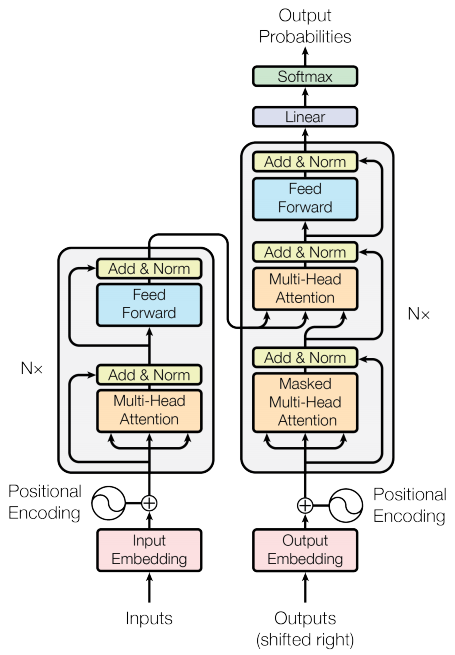
\includegraphics[scale=.4]{img/transformer.png}
\caption{Kiến trúc mô hình Transformer\cite{DBLP:journals/corr/VaswaniSPUJGKP17}}
\label{fig:transformer_diagram}
\end{figure}
\begin{itemize}
\item Câu đầu vào ở ngôn ngữ A được Encoder chuyển thành một ma trận trong không gian ngữ nghĩa bằng cách chuyển mỗi từ trong câu thành một vector biểu diễn (word embedding vector). Dùng cơ chế self-attention, Transformer học ngữ nghĩa của mỗi từ bằng cách xem xét quan hệ của từ với các từ còn lại, từ đó tổng hợp thông tin ngữ nghĩa của câu và tạo ra vector biểu diễn mới thể hiện độ phụ thuộc ngữ nghĩa của từ với ngữ cảnh của câu. Quá trình này được thực hiện song song với cơ chế multi-head attention.
\item Output của Encoder được đưa vào Decoder cùng vector biểu diễn của câu ở ngôn ngữ B, sau đó đưa qua các lớp masked self-attention và cross-attention để tính toán sự liên hệ về ngữ nghĩa giữa 2 vector biểu diễn A và B. Khác với Encoder sử dụng toàn bộ ngữ nghĩa của câu, Decoder chỉ sử dụng ngữ nghĩa từ các token đã có $1, 2, .., t$ để đưa ra dự đoán cho token $t + 1$, dùng cơ chế masked self-attention. Output của Decoder sau đó được đưa qua các lớp Fully Connected và Softmax để đưa ra kết quả.
\end{itemize}
Một số điểm mạnh của Transformer so với các mô hình dịch máy truyền thống bao gồm:
\begin{itemize}
\item Transformer có thể học và ghi nhớ được ngữ nghĩa của các văn bản dài, khác với các mạng dịch máy truyền thống dùng RNN hay LSTM bị phụ thuộc vào độ dài của vẳn bản và không có khả năng ghi nhớ được ngữ nghĩa khi xử lý các văn bản dài.
\item Với khả năng tính toán song song, Transformer trở nên hiệu quả trên phần cứng phục vụ tính toán như GPU hay TPU, khác với các kiến trúc truyền thống.
\end{itemize}

\subsection{BERT}
Phần Encoder của Transformer được sử dụng trong mô hình BERT (\textbf{B}idirectional \textbf{E}ncoder \textbf{R}epresentations from \textbf{T}ransformers)\cite{devlin-etal-2019-bert}. BERT được giới thiệu có 2 phiên bản với các hyperparameters (siêu tham số) và số lượng training parameters (tham số huấn luyện) khác nhau:

\begin{figure}
\centering
\resizebox{\textwidth}{!}
{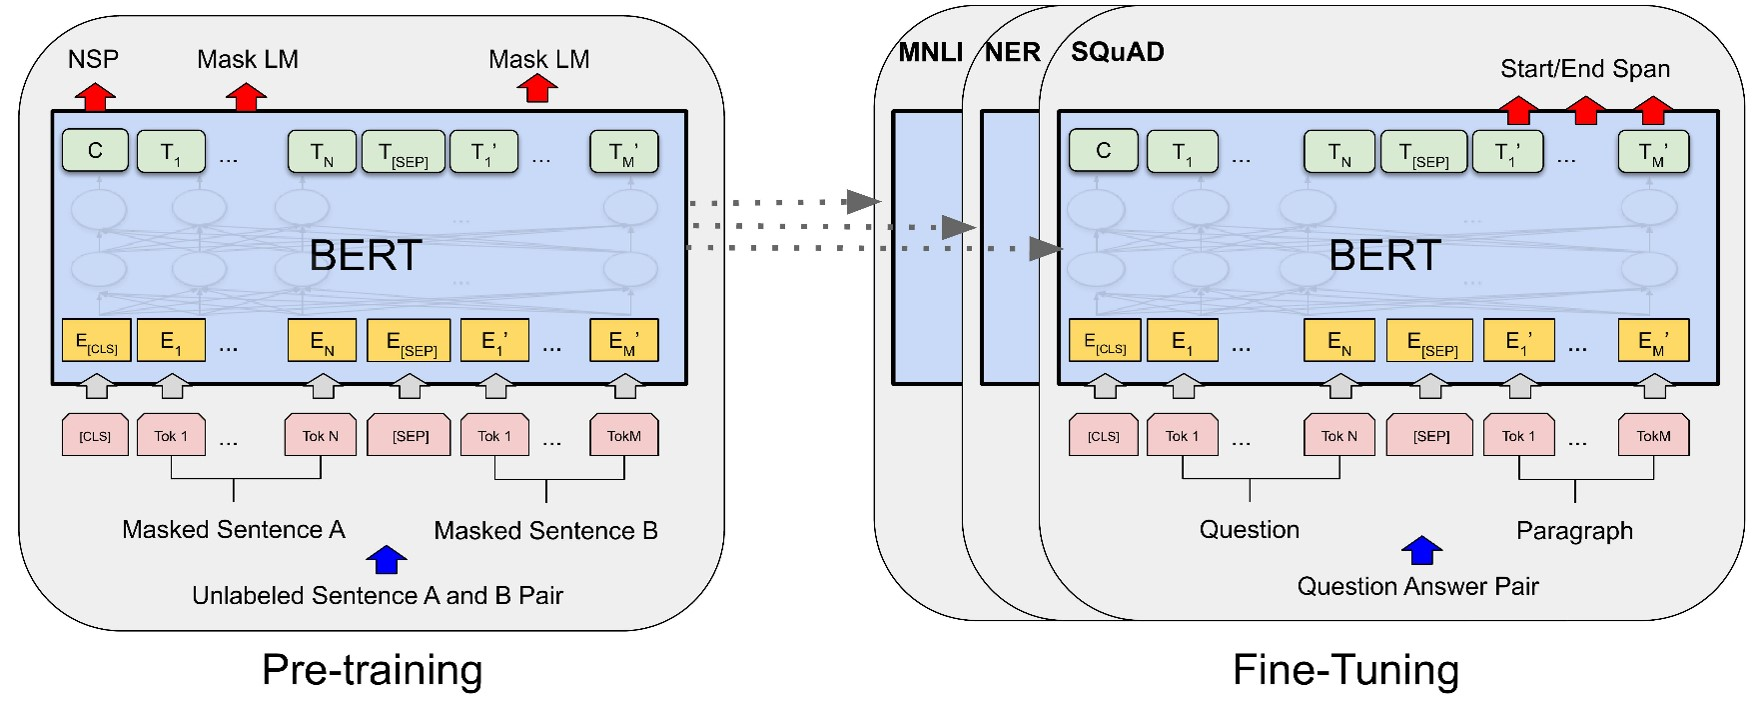
\includegraphics{img/BERT.jpg}}
\caption{Mô hình BERT\cite{devlin-etal-2019-bert}}
\label{fig:my_label}
\end{figure}
\begin{itemize}
\item \textbf{BERT\textsubscript{base}}: 12 Transformer encoder layers, 768 hidden units, 12 attention heads, 110 triệu parameters.
\item \textbf{BERT\textsubscript{large}}: 24 Transformer encoder layers, 1024 hidden units, 16 attention heads và 340 triệu parameters.
\end{itemize}
BERT được tiền huấn luyện (pretrain) với bộ ngữ liệu \textit{BookCorpus} (800 triệu từ) và \textit{Wikipedia English} (2500 triệu từ) với các pretraining task Masked Language Modeling (MLM) và Next Sentence Prediction (NSP):
\begin{itemize}
\item Đầu vào của mô hình BERT là 2 câu $A$ và $B$. Input embedding được tạo bằng cách thêm token \texttt{[CLS]} và \texttt{[SEP]} sao cho token \texttt{[CLS]} đánh dấu vị trí bắt đầu của câu $A$, token \texttt{[SEP]} đánh dấu vị trí kết thúc câu $A$ và bắt đầu câu $B$. Input embedding sau đó được đưa qua segment embedding để đánh dấu token thuộc câu $A$ hay $B$, cuối cùng đưa qua positional embedding để đánh dấu vị trí của token trong câu.

\item \textbf{MLM}: Vector embedding được đưa qua $N$ block Transformer Encoder. BERT sẽ chọn ngẫu nhiên 15\% số lượng token trong input để mask với các chiến lược: 80\% mask token bằng một token đặc biệt, 10\% thay ngẫu nhiên token với một token khác và 10\% giữ nguyên token được chọn. Theo cách này BERT sẽ học được cách dự đoán cho từng token ở các vị trí khác nhau.

\item \textbf{NSP}: Ngữ liệu huấn luyện sẽ đảm bảo 50\% câu $B$ là câu tiếp theo của câu $A$, 50\% còn lại câu $B$ chỉ là một câu ngẫu nhiên được lựa chọn từ bộ ngữ liệu huấn luyện. Vector output $C$ (tương ứng với vị trí token \texttt{[CLS]} trong input) sẽ mang đủ thông tin giúp chúng ta xác định $B$ có phải là câu tiếp theo của $A$ trong một văn cảnh nào đó hay không.
\end{itemize}

Mô hình BERT sau khi huấn luyện sẽ được tinh chỉnh (finetune) lại cho các downstream task khác nhau. Sau khi BERT được công bố, nhiều mô hình cải tiến của BERT cũng được giới thiệu dựa trên kiến trúc của BERT, trong đó có thể kể đến

\begin{itemize}
\item \textbf{RoBERTa} (\textbf{R}obustly \textbf{o}ptimized \textbf{BERT} Pretraining \textbf{a}pproach)\cite{DBLP:journals/corr/abs-1907-11692}: sử dụng dynamic masking so với sử dụng static masking trong kiến trúc gốc; huấn luyện trên nhiều ngữ liệu hơn.
\item \textbf{ALBERT} (\textbf{A} \textbf{L}ight \textbf{BERT})\cite{https://doi.org/10.48550/arxiv.1909.11942}: dùng một số kĩ thuật tối ưu bộ nhớ và tăng tốc độ huấn luyện của BERT.
\item \textbf{DistilBERT}\cite{DBLP:journals/corr/abs-1910-01108}: mô hình nhỏ, nhanh, tốn ít chi phí huấn luyện hơn mô hình BERT gốc: có ít hơn 40\% parameters, chạy nhanh hơn 60\% nhưng hiệu quả bằng 95\% so với mô hình gốc.
\end{itemize}

\subsection{PhoBERT}
Dựa trên mô hình BERT, nhóm nghiên cứu từ VinAI đã công bố PhoBERT\cite{phobert}, được giới thiệu là mô hình ngôn ngữ đơn ngữ quy mô lớn dành cho tiếng Việt đầu tiên. PhoBERT sử dụng quá trình pretraining của RoBERTa để tăng hiệu quả cho mô hình. Kiến trúc của PhoBERT vẫn giữ nguyên so với BERT:
\begin{itemize}
\item \textbf{PhoBERT\textsubscript{base}}: 12 encoder layers, 768 hidden units, 12 attention heads, 135 triệu parameters.
\item \textbf{PhoBERT\textsubscript{large}}: 24 encoder layers, 1024 hidden units, 16 attention heads và 370 triệu parameters.
\end{itemize}
PhoBERT được pretrain với bộ ngữ liệu \textit{Wikipedia Tiếng Việt} và bộ ngữ liệu tin tức tiếng Việt \textit{Binhvq News Corpus}\footnote{\href{https://github.com/binhvq/news-corpus}{https://github.com/binhvq/news-corpus}}.

\subsection{ViHealthBERT}
Mô hình ViHealthBERT sử dụng kiến trúc của BERT (12 encoder layer, 768 hidden units, 12 attention heads) với bộ trọng số huấn luyện của PhoBERT. Việc huấn luyện ViHealthBERT chia làm 2 giai đoạn:
\begin{itemize}
\item \textbf{Giai đoạn pretraining}: Huấn luyện trên các bộ ngữ liệu \textit{Text Mining Corpus} và \textit{OSCAR} : Masked Language Modeling (MLM), Capitalized Prediction (CP) và Next Sentence Prediction (NSP).
\item \textbf{Giai đoạn finetuning}: Finetuning trên các bộ ngữ liệu \textit{PhoNER\_COVID-19, VimQ, arcDrid} và \textit{FAQ Summarization}: Named-Entity Recognition (NER), Acronym Disambiguation và FAQ Summarization
\end{itemize}

\begin{figure}
\begin{center}
\resizebox{\textwidth}{!}{
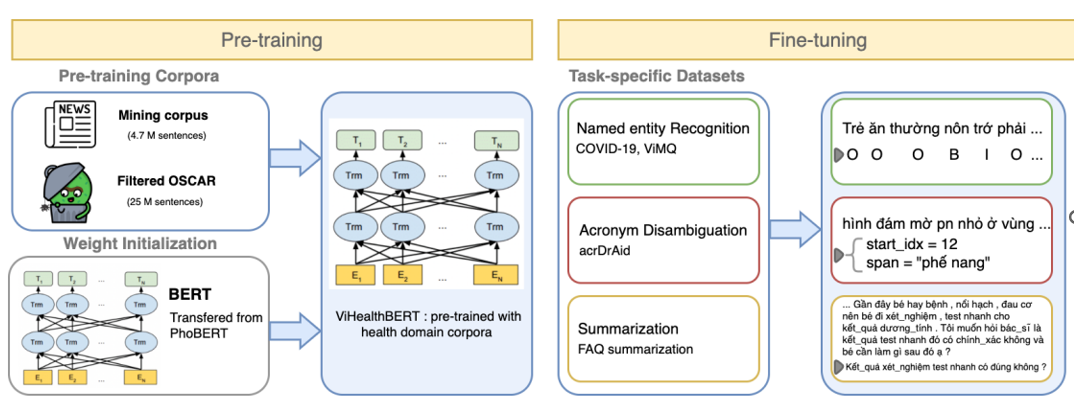
\includegraphics{img/ViHealthBERT.png}
}
\caption{Tổng quan về quá trình pretraining và finetuning trong ViHealthBERT\cite{minh-EtAl:2022:LREC}}
\end{center}
\end{figure}